\section{Introduction}
\label{sec:intro}

With the relentless development of \Gls{AI}, new
architectures and new ways of analyzing texts and images are leading to many new
models. This enthusiasm enables us to meet a wide range of needs but analyzing
all these tools and choosing the right \Gls{AiModel} to best solve your specific
problem is becoming less and less straightforward.

Building a model from scratch for a specific application is time-consuming and
tedious. Numerous public repositories of AI models exist, avoiding this
preliminary work and allowing you to concentrate on use (\Gls{AiInference}) and/or
adjustments (\Gls{AiFineTuning}). It is therefore vital to be able to select the most
accurate \Gls{PreTrainedModel} from those available, if possible, as automatically
as possible.

We want to tackle this problem by lowering the barriers for reusing trained AI
models available in \Gls{AiRepositories}.

\begin{figure}[H]
\centering
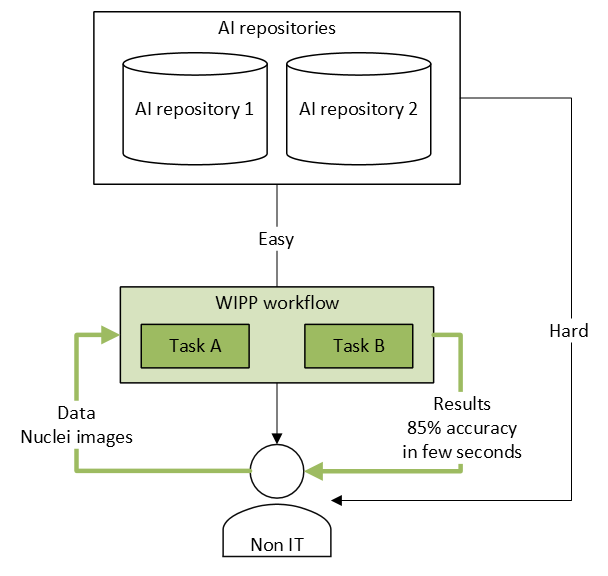
\includegraphics[width=0.8\linewidth]{png/introduction/layman.png}
\caption{Purpose of the work}
\end{figure}

Challenges are numerous: there is no
standard \Gls{API} to access public AI repositories; models are spread on
lot of different repositories and formats; re-train models from scratch take lot
of time and money; for non-technical researchers, it is not trivial to setup and
execute AI models; there is insufficient metadata about trained AI models in
public AI repositories to match them to applications and to run them; there
is no way of automatically assessing the accuracy of AI models.

Our motivations with this work is to accelerate application of AI models to
scientific problems and save hours of computation time by reusing pre-trained
models from diverse repositories.




